\documentclass[11pt,a4paper]{report}
\usepackage[margin=25mm]{geometry}
\usepackage{amsmath}
\usepackage{booktabs}
\usepackage{graphicx}
\usepackage{float}
\usepackage[hidelinks]{hyperref}
\usepackage{xcolor}
\setlength{\parindent}{0pt}
\setlength{\parskip}{0.65em}
\newcommand{\measured}{\textbf{Measured}}
\newcommand{\simulated}{\textbf{Simulated}}

\begin{document}

\begin{titlepage}
\centering
{\large UNIVERSITY OF MARIBOR\\FACULTY OF ELECTRICAL ENGINEERING AND COMPUTER SCIENCE\\UM FERI\par}
\vspace{2.5cm}
{\Huge\bfseries 1-DOF Series-Elastic Finger Exoskeleton\par}
\vspace{0.4cm}
{\Large Actuator Commissioning, Embedded Control, sEMG Intent Detection, and Virtual SEA Evaluation\par}
\vfill
\begin{tabular}{ll}
Institutional mentor: & Prof. dr. Ale\v{s} Hace\\
Prepared by: & Drin Duka\\
Date: & 8 July 2026
\end{tabular}
\vfill
{Maribor, 2026\par}
\end{titlepage}

\begin{abstract}
This project investigated a one-degree-of-freedom series-elastic-actuated (SEA) finger exoskeleton for surface-electromyography (sEMG) intent detection and later sensorimotor analysis. The available Harmonic Drive PMA-8A actuator, Maxon ESCON 50/5 controller, incremental encoder, and STM32 NUCLEO-F446RE were commissioned. Closed-loop low-speed rotation was first verified using the ESCON potentiometer and then commanded by STM32 analog and digital outputs. A laptop bridge was implemented to acquire eight-channel Myo armband EMG and inertial data, calibrate a repeatable pinch-intent template, reject competing gestures and motion, log trials, and communicate with the STM32 over serial.

The physical spring, tendon transmission, finger mechanism, and spring-deflection sensor were unavailable and therefore were not represented as completed hardware. Instead, recorded real EMG classification was replayed through an explicitly labelled virtual SEA model to demonstrate the intended bounded $0$--$180^\circ$ motion and the relationship between spring deflection and force. The result is a validated physical actuator-and-embedded-control MVP, a separately validated sEMG intent subsystem, and a reproducible simulation of the missing compliant mechanism. Physical Myo-to-actuator operation, impedance control, and electromechanical-delay measurement remain future integration work.
\end{abstract}

\tableofcontents

\chapter{Objective and Scope}

The declared research objective was a 1-DOF dorsal finger exoskeleton driven through a series elastic element. The intended control and sensing chain was
\[
\text{sEMG intent}\rightarrow\text{embedded controller}\rightarrow\text{motor}\rightarrow
\text{spring/tendon}\rightarrow\text{finger motion}.
\]
The proposed series spring had stiffness $k_s\approx2.0\,\mathrm{N/mm}$. Its measured deflection would provide an indirect force estimate,
\begin{equation}
F_s=k_s\Delta x_s,
\end{equation}
and, after mechanism calibration, an interaction torque estimate. The intended impedance law was
\begin{equation}
\tau_{cmd}=K_v(\theta_{target}-\theta)+B_v(\omega_{target}-\omega).
\end{equation}

The final available hardware did not include the spring, Bowden/tendon transmission, displacement sensor, or printed finger mechanism. Consequently, this report distinguishes three evidence classes:
\begin{itemize}
  \item \measured: voltages, ESCON monitor values, EMG, IMU, and serial responses;
  \item \textbf{Observed}: physical actuator motion in photographs and videos;
  \item \simulated: finger angle, spring deflection, spring force, and virtual SEA dynamics.
\end{itemize}
No simulated signal is presented as a physical measurement.

\chapter{Physical System}

\section{Hardware architecture}

The physical test bench comprised a PMA-8A-50-01-E500ML actuator, ESCON 50/5, incremental encoder, NUCLEO-F446RE, and an external DC supply. The ESCON handled encoder-based closed-loop velocity control. The STM32 supplied only the speed setpoint and enable signal.

\begin{table}[H]
\centering
\caption{Verified STM32-to-ESCON interface.}
\begin{tabular}{lll}
\toprule
STM32 signal & ESCON connection & Function\\
\midrule
PA4 / A2 & J6 pin 1, Analog Input 1+ & Analog speed setpoint\\
GND & J6 pin 2, Analog Input 1-- & Analog reference\\
PC0 / A5 & J5 pin 2, Digital Input 2 & High-active enable\\
GND & J5 pin 5, Signal GND & Digital reference\\
\bottomrule
\end{tabular}
\end{table}

\begin{figure}[H]
\centering
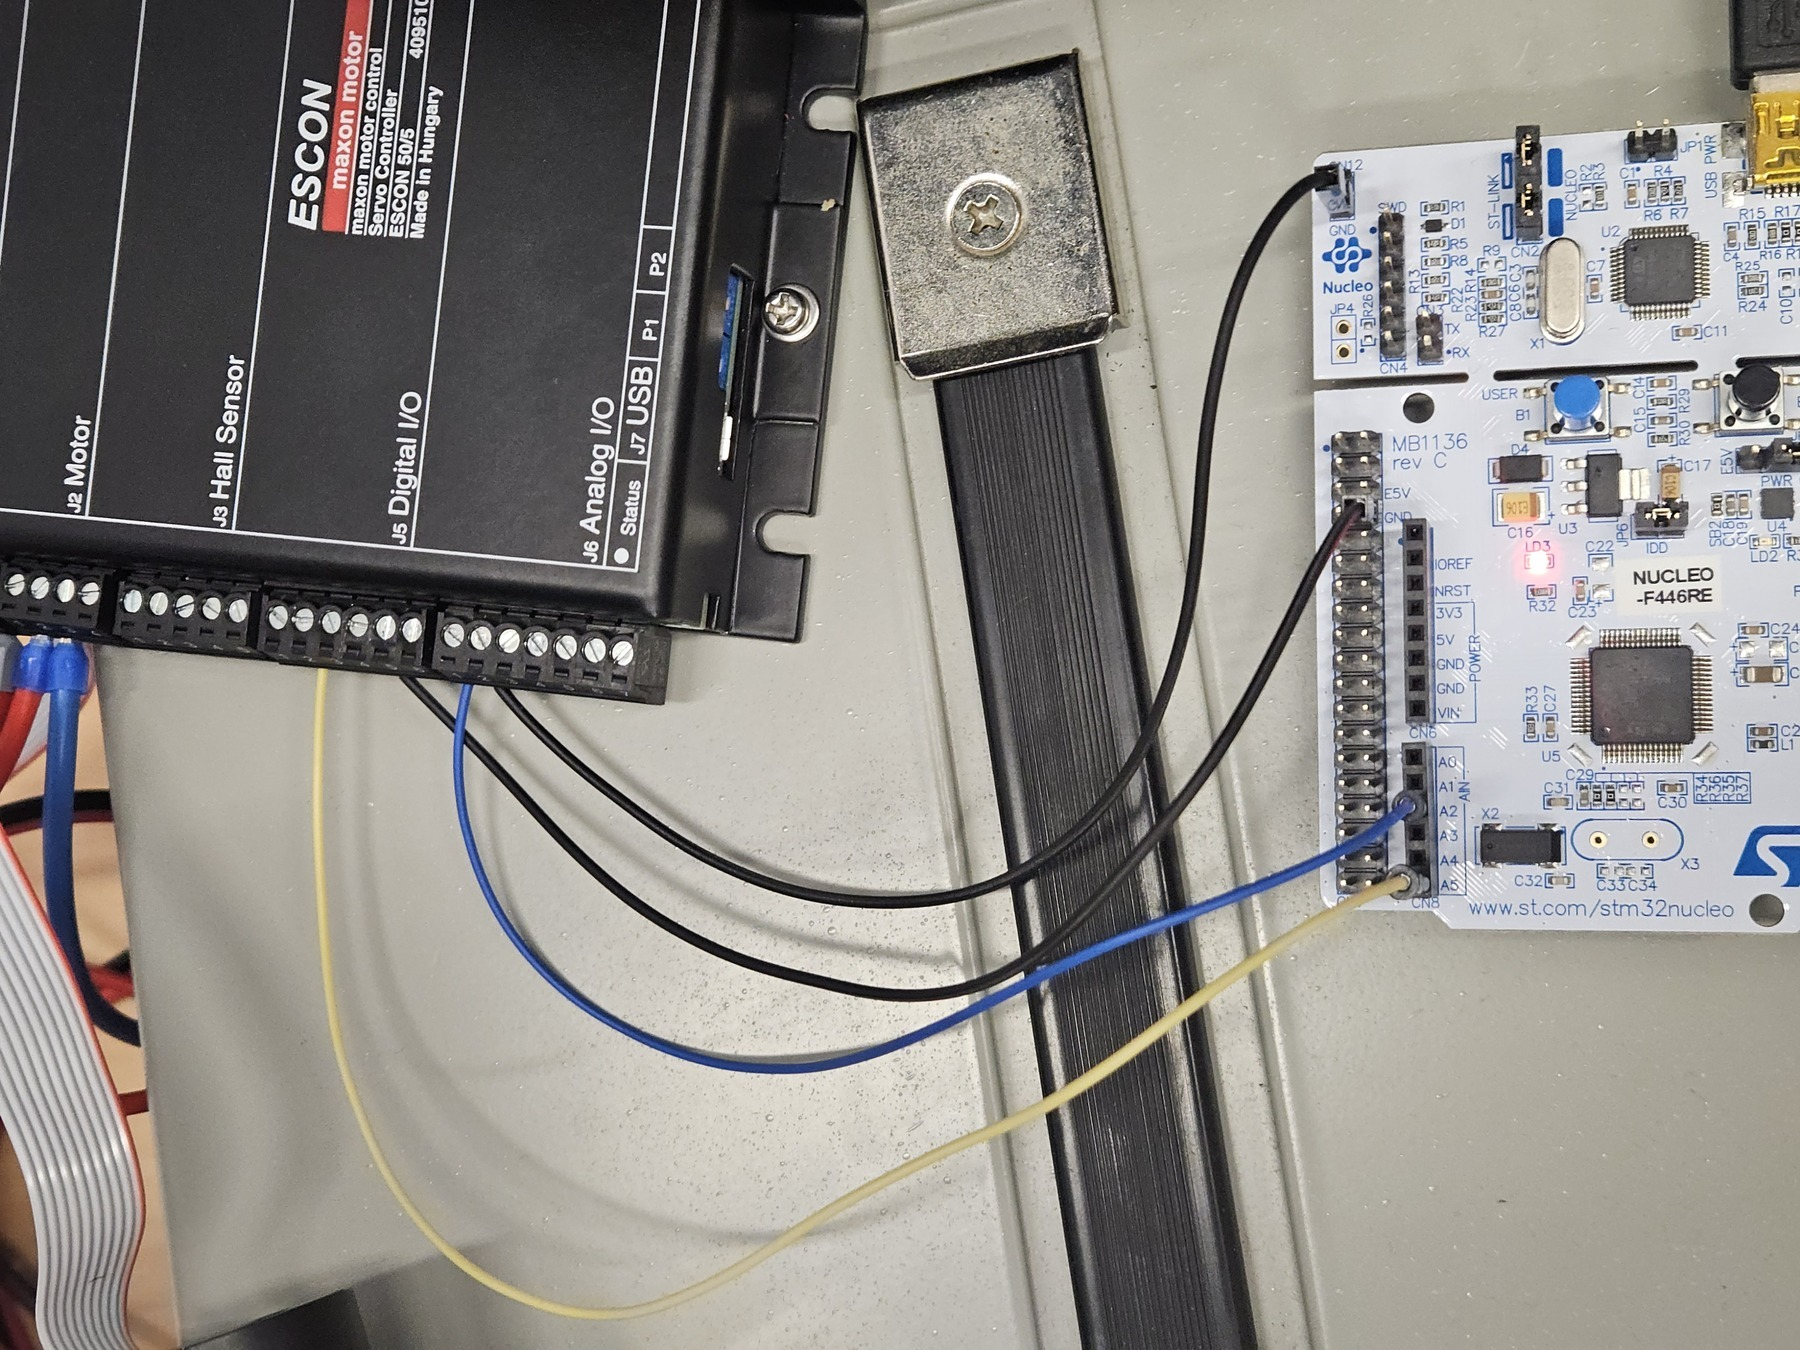
\includegraphics[width=0.92\textwidth]{figures/stm32-escon-wiring.jpg}
\caption{Observed STM32-to-ESCON signal wiring. The photograph documents the physical command interface, not a completed finger mechanism.}
\end{figure}

\section{ESCON configuration and commissioning}

The ESCON was configured as a closed-loop speed controller with a 500-pulse digital incremental encoder. Initial limits were deliberately conservative.

\begin{table}[H]
\centering
\caption{Commissioning configuration recovered from the final ESCON file.}
\begin{tabular}{ll}
\toprule
Parameter & Value\\
\midrule
Controller & Maxon ESCON 50/5\\
Control mode & Closed-loop speed control\\
Setpoint source & Analog Input 1\\
Setpoint scaling & $0\,\mathrm{V}\rightarrow0\,\mathrm{rpm}$; $1\,\mathrm{V}\rightarrow100\,\mathrm{rpm}$\\
Enable & Digital Input 2, high-active\\
Encoder & Digital incremental, 500 pulses/revolution\\
Nominal current & $0.60\,\mathrm{A}$\\
Maximum output current & $1.00\,\mathrm{A}$\\
Acceleration/deceleration & $100\,\mathrm{rpm/s}$\\
Maximum permissible speed & $6000\,\mathrm{rpm}$\\
\bottomrule
\end{tabular}
\end{table}

Supervised automatic tuning completed successfully. Stable rotation was first observed using Potentiometer~1. The STM32 interface was then verified independently with a multimeter before connection to the ESCON. The measured active outputs were approximately $1.00\,\mathrm{V}$ on PA4 and $3.31\,\mathrm{V}$ on PC0; inactive output was approximately $0.00\,\mathrm{V}$.

\begin{figure}[H]
\centering
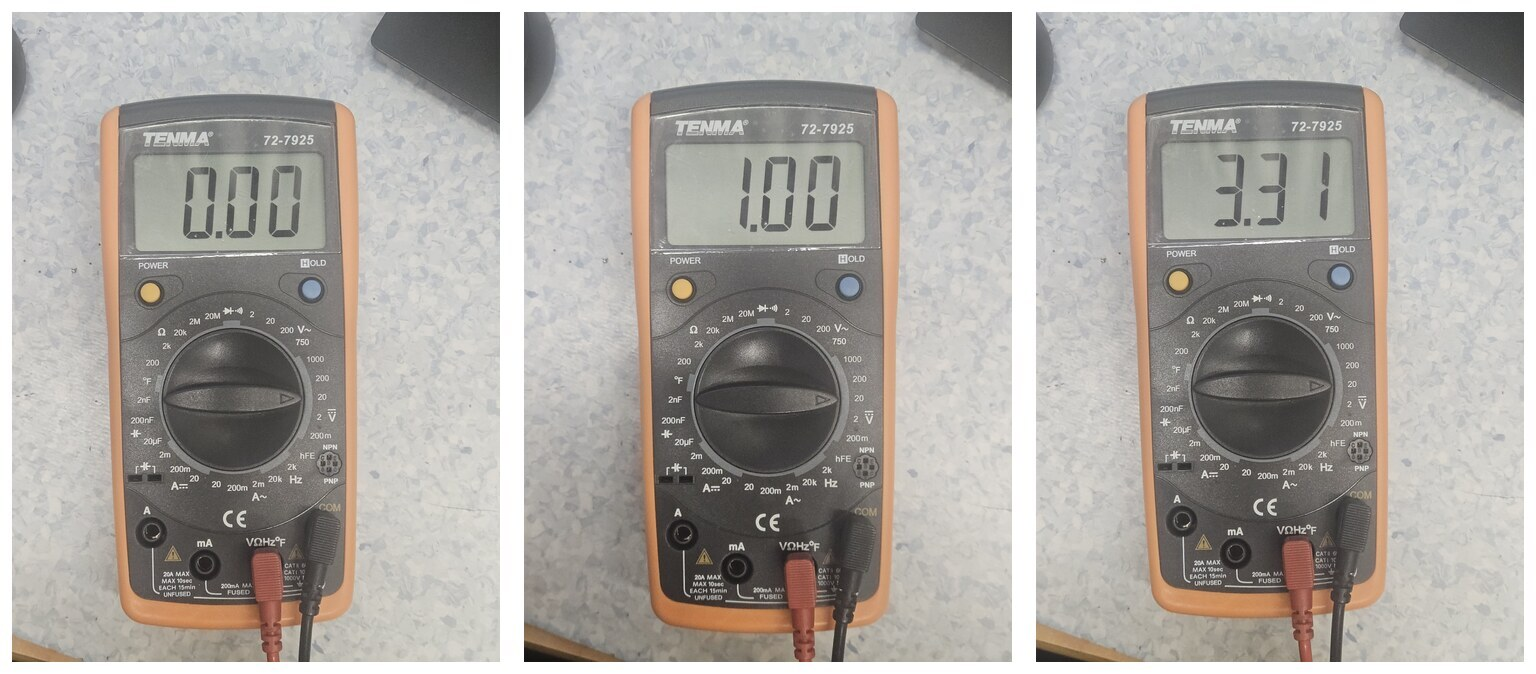
\includegraphics[width=\textwidth]{figures/stm32-output-measurements.jpg}
\caption{Measured STM32 command voltages before connection to the motor controller: inactive DAC (left), active DAC (centre), and active digital enable (right).}
\end{figure}

Pressing the Nucleo user button asserted enable and the $1$ V command; ESCON Studio showed demand and actual speeds near $100$ rpm, and the actuator rotated stably. Releasing the button returned the DAC to $0$ V, removed enable, and stopped the actuator. Repeated start/stop operation was recorded on video. This is the completed physical MVP.

\chapter{sEMG Intent Detection}

\section{Acquisition and features}

The deprecated Myo armband was connected to a laptop over BLE. The laptop subscribed to eight EMG channels and IMU data. No Bluetooth discovery was required during normal use because the known device address was supplied directly. For each $200$ ms sliding window with a $50$ ms step, the mean absolute value (MAV) was calculated:
\begin{equation}
f_i=\frac{1}{N}\sum_{n=1}^{N}|e_i[n]|,\qquad i=1,\ldots,8.
\end{equation}
Total activity and the normalized spatial pattern were
\begin{equation}
A=\sum_i f_i,\qquad p_i=\frac{f_i}{A+\epsilon}.
\end{equation}

\section{Calibration and classification}

Calibration recorded rest in three forearm orientations, several candidate intents, static rejection gestures, and wrist/forearm motion. Candidate intents were ranked by within-class cosine similarity minus their strongest rejection similarity. The selected pinch attempt was retained only when it produced sufficient activity above rest and a repeatable spatial pattern.

Live classification required activity above the orientation-specific rest threshold, adequate target similarity, a positive margin over the strongest rejection class, and low gyroscope magnitude. Hysteresis and hold times suppressed rapid switching. The detector states were REST, TARGET, GESTURE\_REJECT, and MOTION\_REJECT. TARGET generated serial command \texttt{1}; all other states generated \texttt{0}. A three-second STM32 command timeout and repeated STOP commands provided communication fail-safe behaviour.

Calibration presets can be reused, numerically adjusted, or partially retaken. Every run logs timestamped raw EMG, MAV features, similarity scores, state, command, IMU magnitude, and virtual-model outputs to CSV.

\chapter{Virtual SEA Replay}

\section{Purpose and assumptions}

The virtual model demonstrates the missing compliant mechanism without claiming physical validation. It replays a real recorded Myo session. Pinch intent commands a target of $0^\circ$ and non-target/relaxed state commands $180^\circ$. Motion is bounded to this interval and rate-limited to $90^\circ/\mathrm{s}$.

The virtual motor angle follows the command subject to the rate limit. Finger angle follows motor angle with a first-order time constant $\tau=0.18$ s. With an assumed $8$ mm tendon moment arm,
\begin{align}
x_m &= r(\theta_{max}-\theta_m),\\
x_f &= r(\theta_{max}-\theta_f),\\
\Delta x_s &= |x_m-x_f|,\\
F_s &= \min(k_s\Delta x_s,F_{max}),
\end{align}
where angular quantities are converted to radians, $k_s=2.0\,\mathrm{N/mm}$, and $F_{max}=5$ N. These values are adjustable simulation parameters, not identified properties of an assembled mechanism.

\section{Replay result}

\begin{figure}[H]
\centering
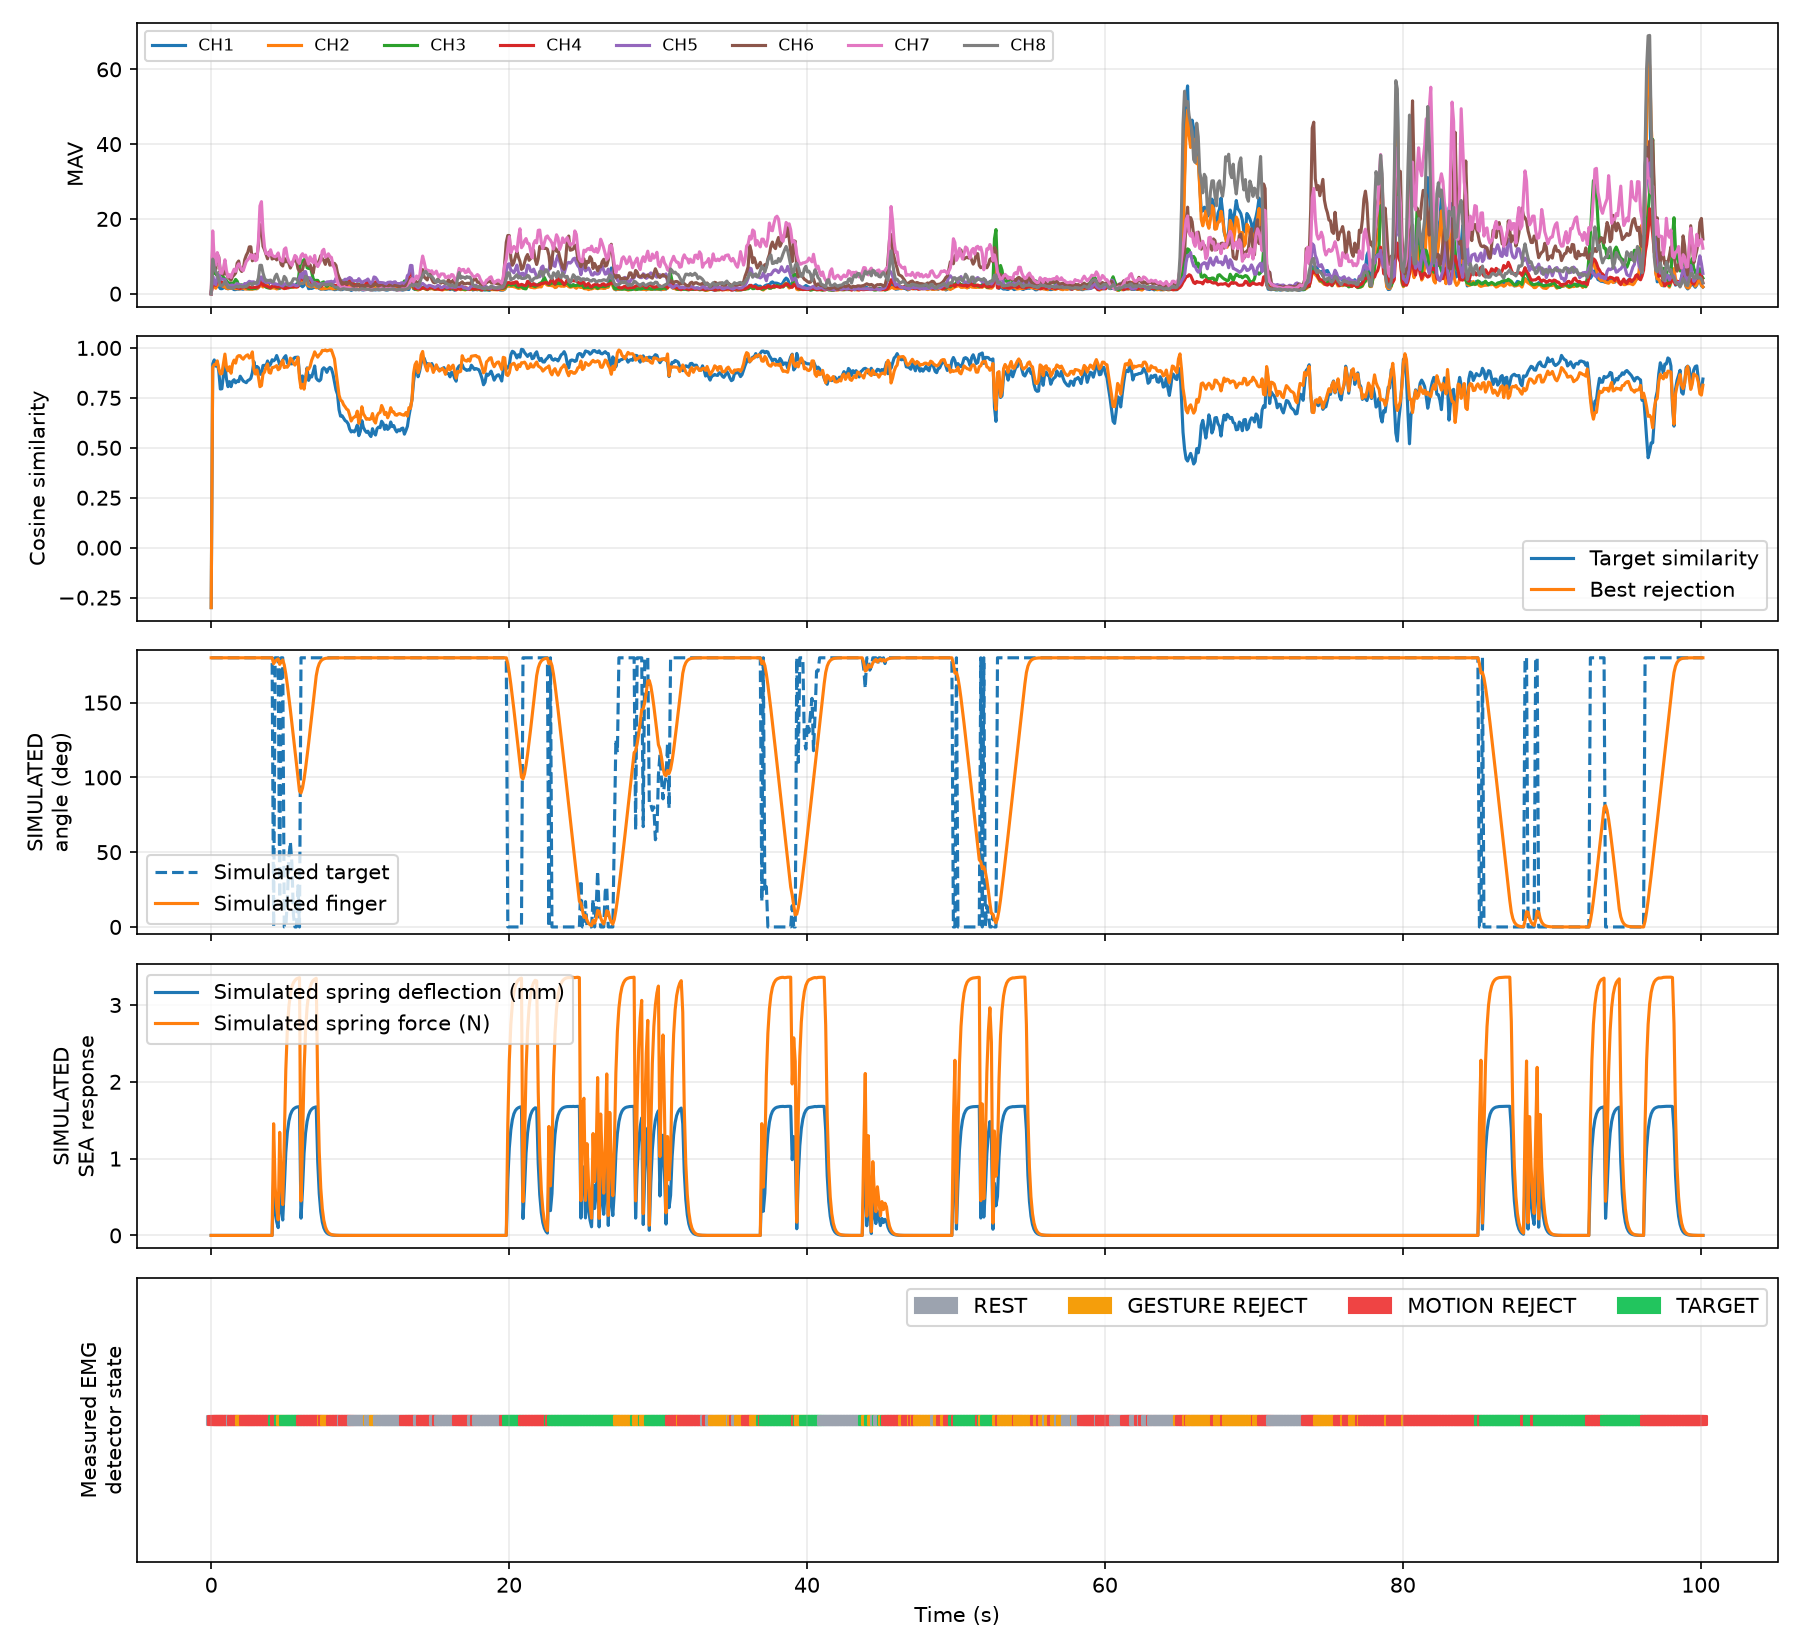
\includegraphics[width=\textwidth]{figures/myo-sea-replay.png}
\caption{Replay of recorded real Myo data. MAV, cosine similarities, and detector states are measured/processed data. Finger angle, spring deflection, and force are explicitly simulated.}
\end{figure}

The replay shows that accepted pinch intervals produce bounded virtual flexion while rejected gestures and high-motion intervals do not sustain the flexion command. Transient motor--finger displacement produces virtual spring deflection and force. This verifies software data flow and intended qualitative behaviour; it does not validate physical impedance, force accuracy, or human interaction safety.

\chapter{Results and Limitations}

\begin{table}[H]
\centering
\caption{Status against the declared study.}
\begin{tabular}{p{0.38\textwidth}p{0.18\textwidth}p{0.34\textwidth}}
\toprule
Item & Status & Evidence\\
\midrule
Actuator and ESCON commissioning & Completed & Tuning, potentiometer motion, monitor screenshots, video\\
STM32 analog command and enable & Completed & Multimeter measurements, wiring photographs\\
STM32-controlled motor motion & Completed & Repeated button start/stop video\\
Myo acquisition and intent detection & Completed diagnostically & Calibration, terminal output, CSV logs, plots\\
Laptop--STM32 serial protocol & Completed on bench & ACK/STATUS transcript and fail-safe firmware\\
Physical Myo-to-motor experiment & Not performed & Kept disabled pending controlled safety test\\
Spring, tendon, and finger mechanism & Not implemented & Components unavailable\\
Spring-deflection force sensing & Simulated only & Virtual replay\\
1 kHz physical impedance control & Not implemented & Requires complete SEA sensing and mechanics\\
EMD/reflex experiment & Not performed & Requires measured spring-force onset and approved protocol\\
\bottomrule
\end{tabular}
\end{table}

The ESCON is a velocity controller, not an absolute-position controller. Its internal encoder closes the velocity loop but does not provide the STM32 with verified finger angle. Therefore the present physical system cannot safely claim $0$--$180^\circ$ finger positioning. A physical SEA requires the compliant element, a calibrated deflection sensor, mechanism geometry, travel limits, and preferably independent output-position sensing.

\chapter{Conclusion and Future Work}

The project established a reproducible actuator-control baseline and extended it with calibrated Myo intent detection. The physical MVP proves that the STM32 can safely command the ESCON and PMA actuator. The software MVP proves that a repeatable pinch intent can be separated from rest, competing gestures, and high-motion activity for this user. The replay connects recorded EMG intent to an explicitly virtual compliant finger model while preserving the boundary between evidence and simulation.

The next engineering step is mechanical rather than algorithmic: fabricate the 1-DOF finger and tendon path, select and calibrate the spring-deflection sensor, add output travel sensing or hard limits, and only then implement and tune the physical impedance loop. EMD measurement should follow validation of synchronized EMG and measured spring-force onset.

\appendix
\chapter{Reproduction Commands}

Run the Myo system without a motor command:
\begin{verbatim}
.venv/bin/python run_myo_sea_demo.py \
  --myo-address D4:71:C5:FF:86:F3 \
  --motor disable --mode diagnostic --live-plot
\end{verbatim}

Generate the measured/simulated replay figure:
\begin{verbatim}
MPLBACKEND=Agg .venv/bin/python plot_log.py logs/SESSION.csv \
  --output report/figures/myo-sea-replay.png
\end{verbatim}

Run the software checks:
\begin{verbatim}
.venv/bin/python -m unittest -v
.venv/bin/python sea_model.py
\end{verbatim}

\begin{thebibliography}{9}
\bibitem{pratt1995} G. A. Pratt and M. M. Williamson, ``Series Elastic Actuators,'' \emph{IEEE/RSJ IROS}, 1995.
\bibitem{hogan1985} N. Hogan, ``Impedance Control: An Approach to Manipulation,'' \emph{Journal of Dynamic Systems, Measurement, and Control}, 1985.
\bibitem{escon} Maxon Motor AG, \emph{ESCON 50/5 Hardware Reference}, document 409510.
\end{thebibliography}

\end{document}
